\documentclass{beamer}

\usepackage[spanish]{babel}
\usetheme{Boadilla}

\title{Clasificación No Supervisada}
\author{Marco Ciccalè Baztán}
\institute{UPM}
\date{\today}

\begin{document}

% Primera slide
\begin{frame}
  \titlepage
\end{frame}

% Introducción
\begin{frame}{Introducción}
  \frametitle{Problema a Resolver}
  \centering
  \begin{figure}
    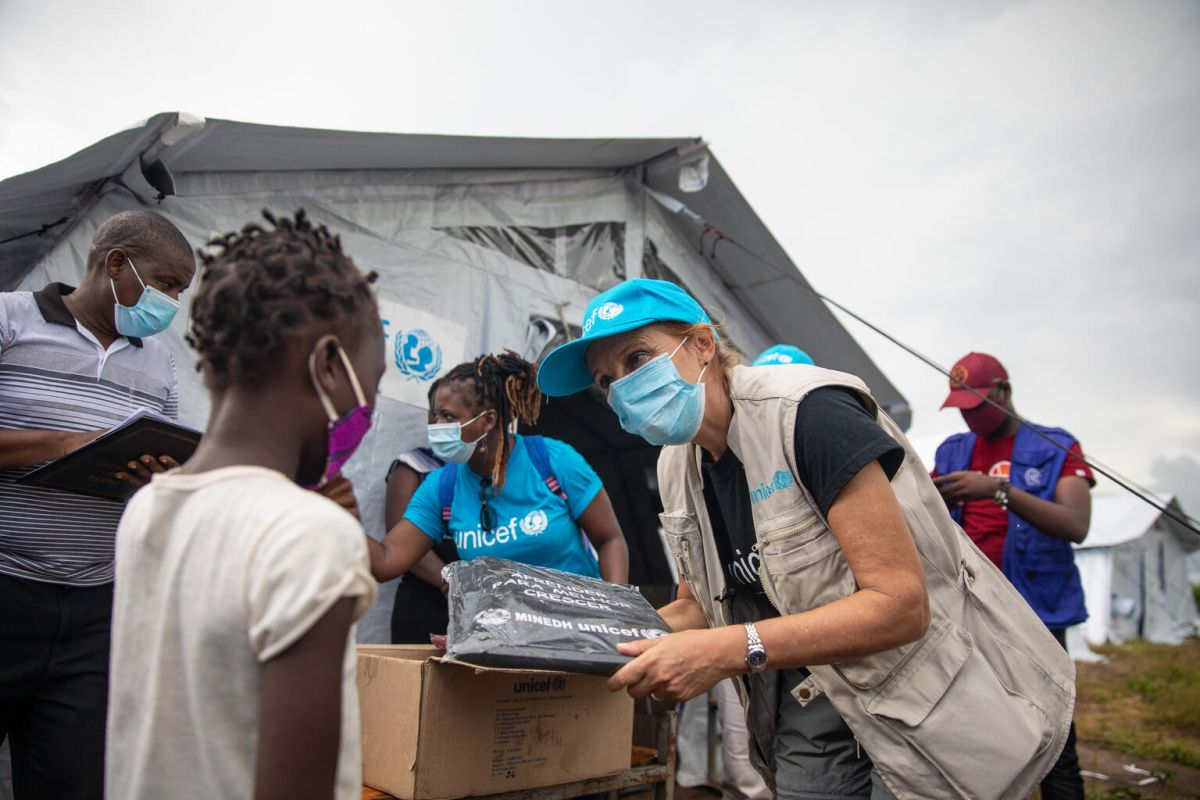
\includegraphics[width=0.8\textwidth]{../images/slides/ayuda-humanitaria.jpg}
  \end{figure}
  Ayuda Humanitaria.
\end{frame}

% Dataset
\begin{frame}{Dataset}
  \frametitle{Dataset}
  \begin{itemize}
    \item 167 países
    \pause
    \item 10 variables: country\pause, child\_mort\pause, exports\pause, health\pause, imports\pause, income\pause, inflation\pause, life\_expec\pause, total\_fer\pause, gdpp.
  \end{itemize}
\end{frame}

\begin{frame}{Dataset2}
  \frametitle{Dataset}
  \centering
  \begin{figure}
    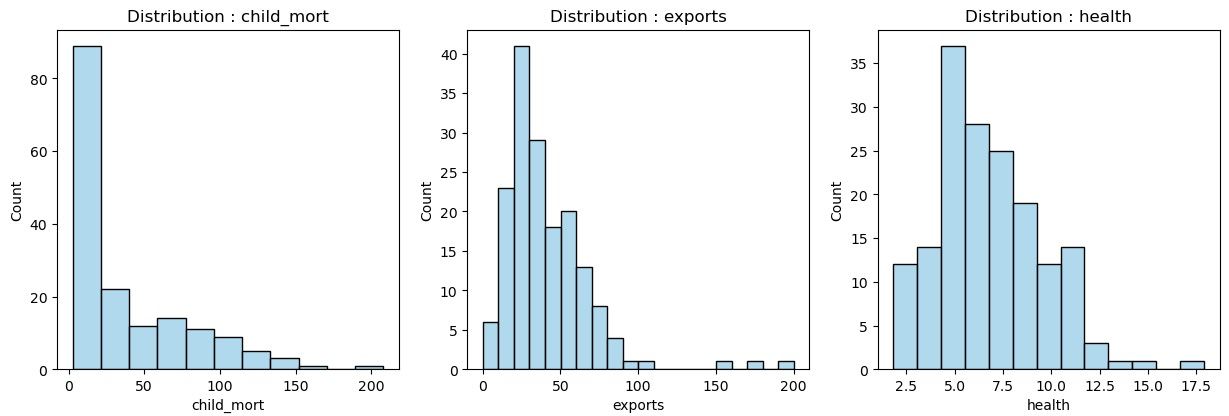
\includegraphics[width=\textwidth]{../images/data/features-analysis-1.jpg}
  \end{figure}
\end{frame}

\begin{frame}{Dataset3}
  \frametitle{Dataset}
  \centering
  \begin{figure}
    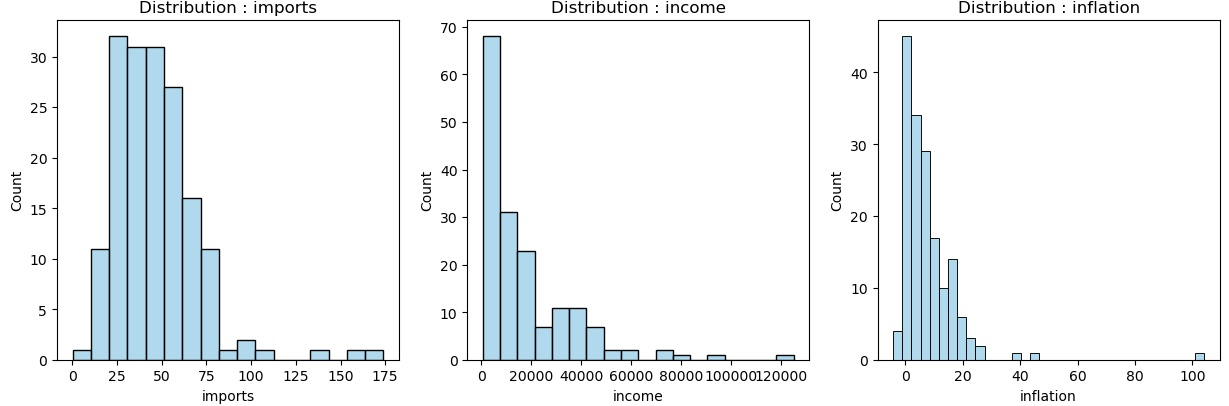
\includegraphics[width=\textwidth]{../images/data/features-analysis-2.jpg}
  \end{figure}
\end{frame}

\begin{frame}{Dataset4}
  \frametitle{Dataset}
  \centering
  \begin{figure}
    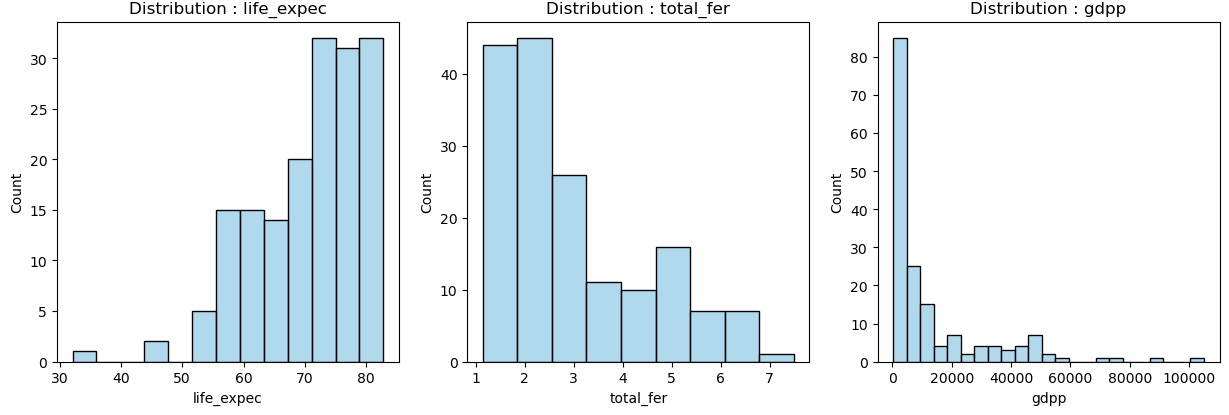
\includegraphics[width=\textwidth]{../images/data/features-analysis-3.jpg}
  \end{figure}
\end{frame}

% Preprocesado de los datos
\begin{frame}{Preprocessing}
  \frametitle{Preprocesado de los Datos}
  \centering
  $\hbox{Diferentes escalas} \rightarrow \pause \hbox{Diferente peso al calcular distancias}$
  \pause

  \vspace{30pt}
  \textit{MaxAbsScaler}
\end{frame}

% Resultados KMeans
\begin{frame}{ResultsKMeans}
  \frametitle{Resultados de KMeans}
  \begin{figure}
    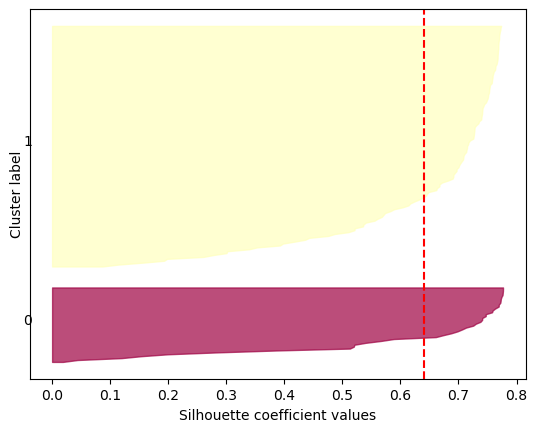
\includegraphics[width=0.8\textwidth]{../images/kmeans/silhouette.png}
  \end{figure}
\end{frame}

\begin{frame}{ResultsKMeans2}
  \frametitle{Resultados de KMeans}
  \begin{figure}
    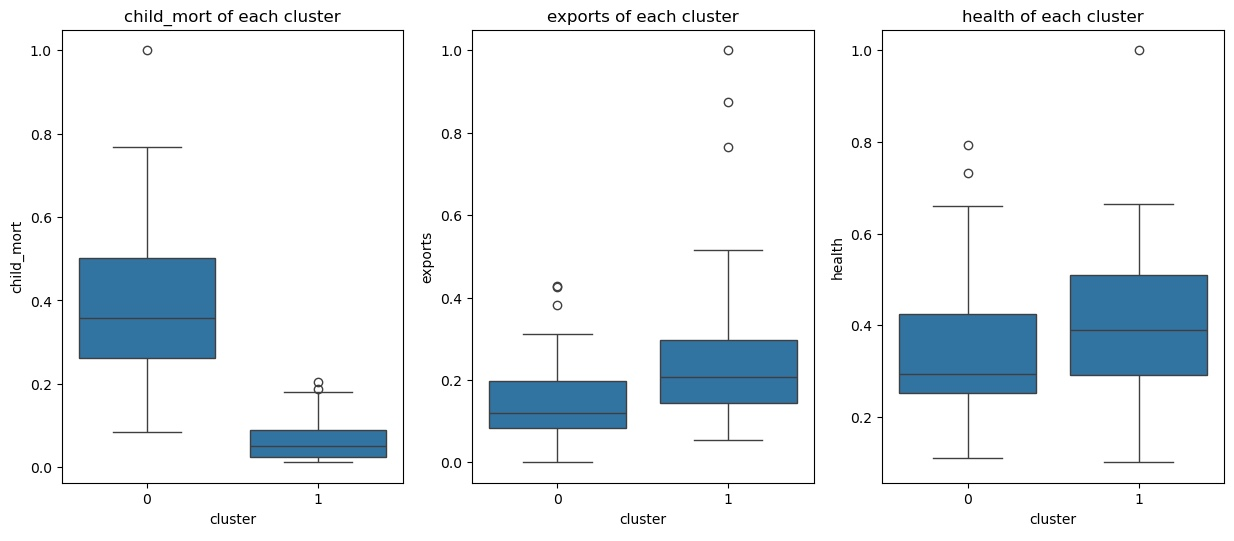
\includegraphics[width=\textwidth]{../images/kmeans/features-dist-1.jpg}
  \end{figure}
\end{frame}

\begin{frame}{ResultsKMeans3}
  \frametitle{Resultados de KMeans}
  \begin{figure}
    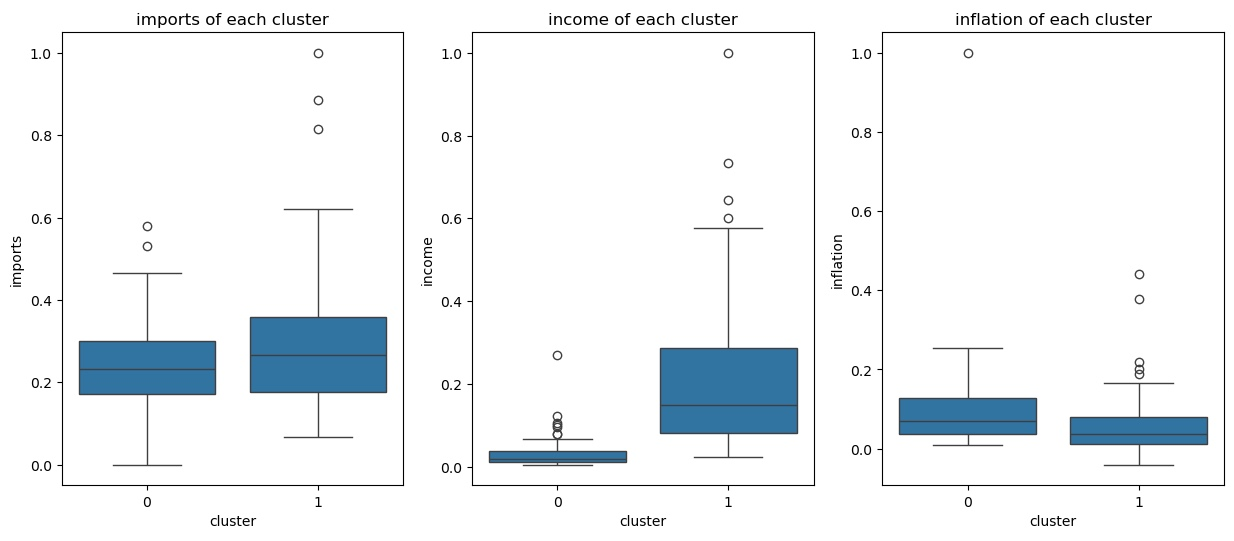
\includegraphics[width=\textwidth]{../images/kmeans/features-dist-2.jpg}
  \end{figure}
\end{frame}

\begin{frame}{ResultsKMeans4}
  \frametitle{Resultados de KMeans}
  \begin{figure}
    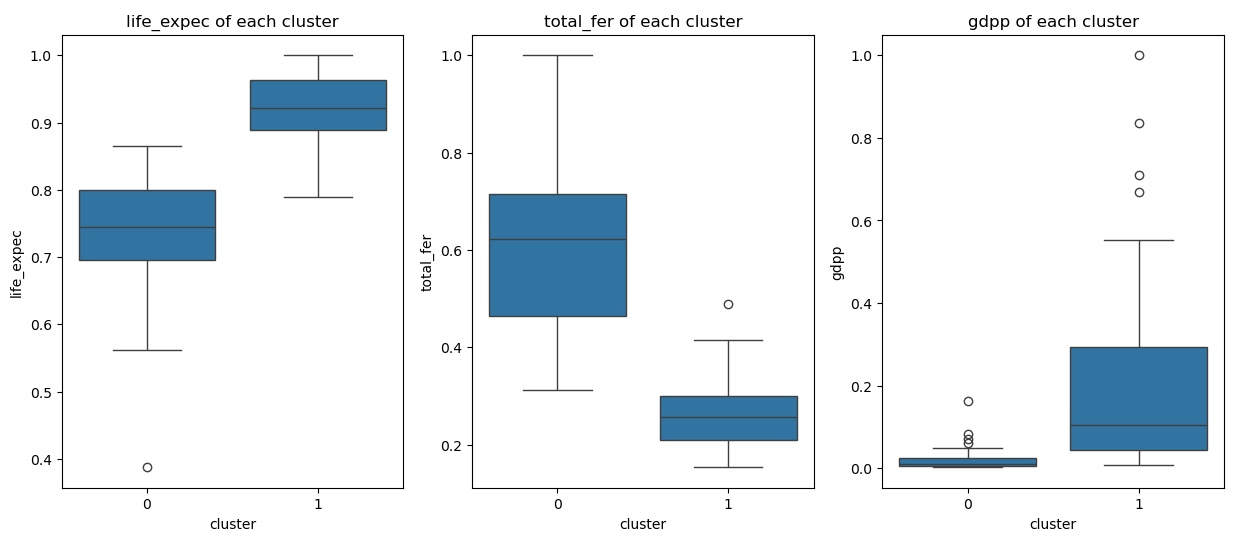
\includegraphics[width=\textwidth]{../images/kmeans/features-dist-3.jpg}
  \end{figure}
\end{frame}

\begin{frame}{ResultsKMeans5}
  \frametitle{Resultados de KMeans}
  \centering
  \begin{figure}
    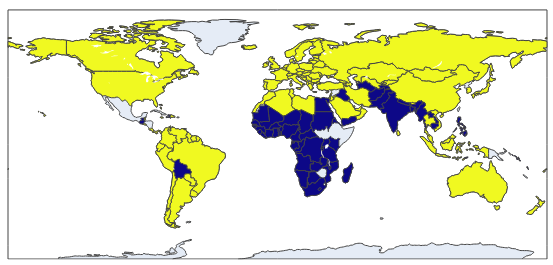
\includegraphics[width=0.8\textwidth]{../images/kmeans/map-cropped.png}
  \end{figure}
  Cluster 0: Azul; Cluster 1: Amarillo
\end{frame}

% Resultados Agglomerative Clustering
\begin{frame}{ResultsAggl}
  \frametitle{Resultados de Agglomerative Clustering}
  \begin{figure}
    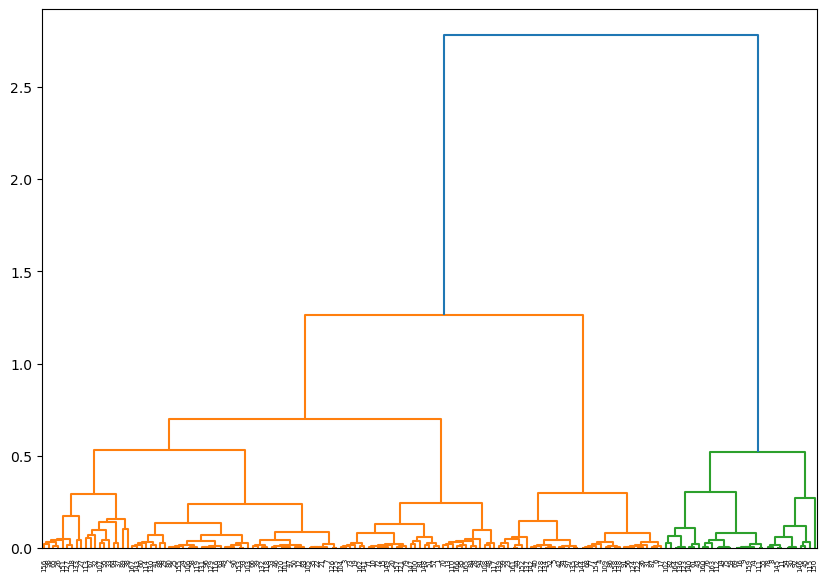
\includegraphics[width=0.8\textwidth]{../images/agglomerative/dendogram.png}
  \end{figure}
\end{frame}

\begin{frame}{ResultsAggl}
  \frametitle{Resultados de Agglomerative Clustering}
  \begin{figure}
    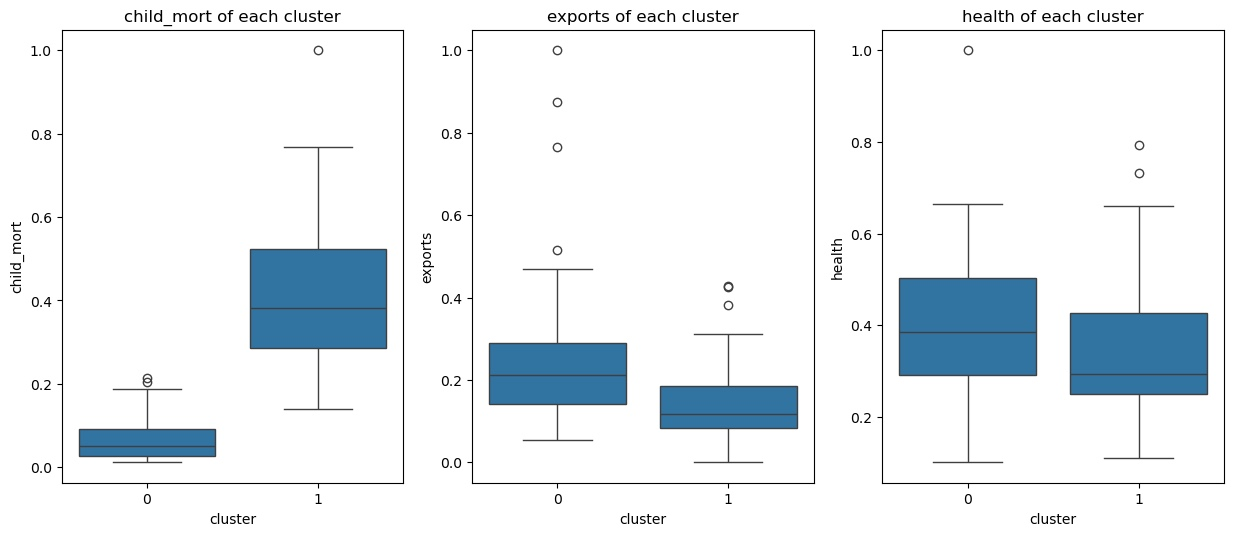
\includegraphics[width=\textwidth]{../images/agglomerative/features-dist-1.jpg}
  \end{figure}
\end{frame}

\begin{frame}{ResultsAggl}
  \frametitle{Resultados de Agglomerative Clustering}
  \begin{figure}
    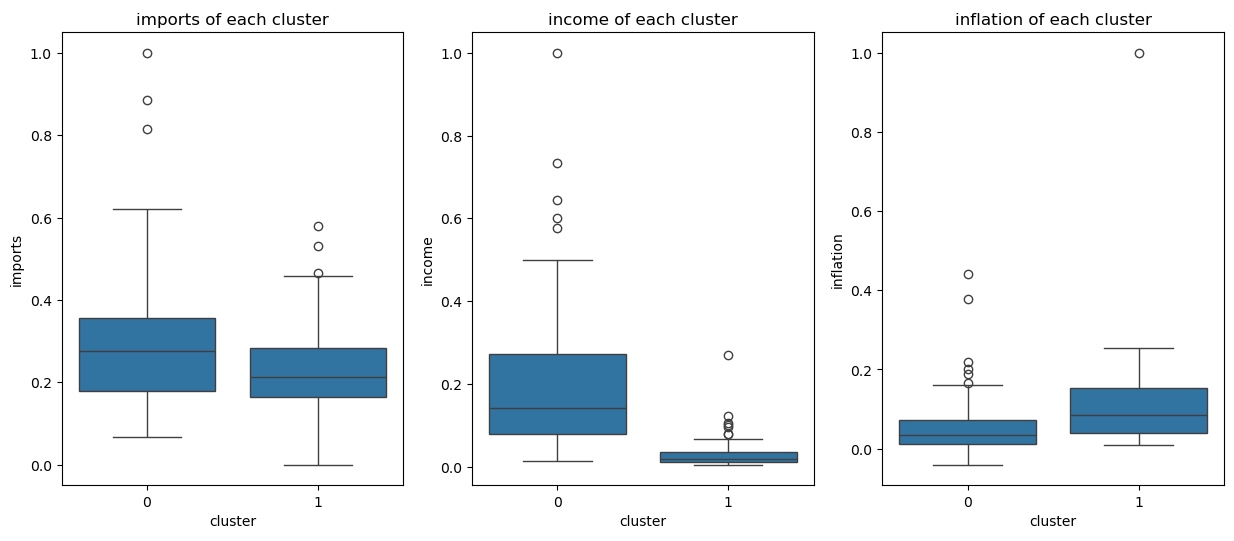
\includegraphics[width=\textwidth]{../images/agglomerative/features-dist-2.jpg}
  \end{figure}
\end{frame}

\begin{frame}{ResultsAggl}
  \frametitle{Resultados de Agglomerative Clustering}
  \begin{figure}
    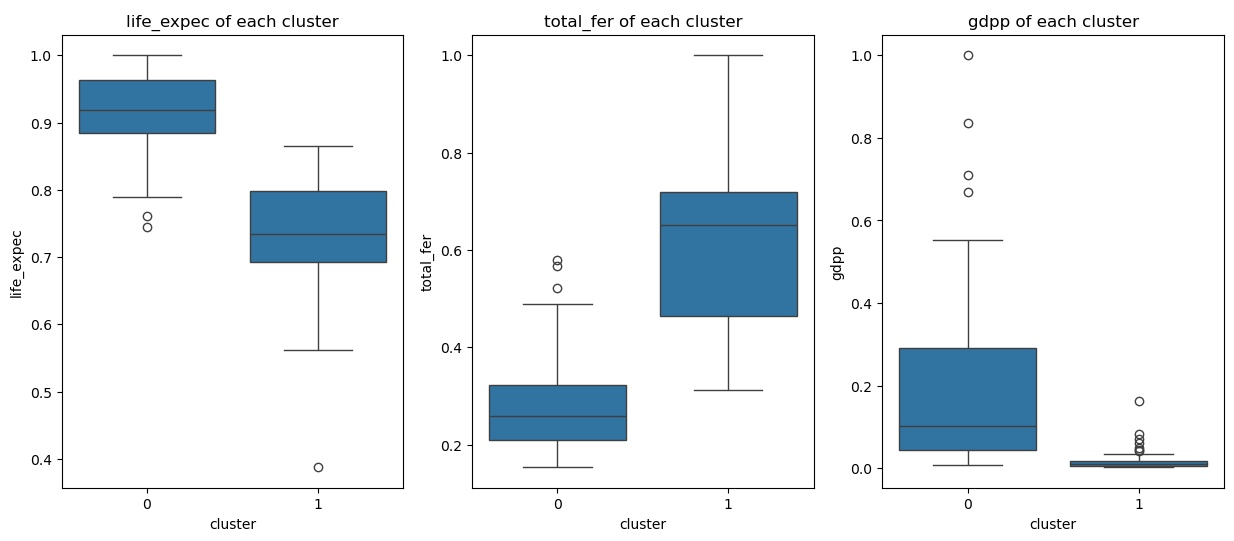
\includegraphics[width=\textwidth]{../images/agglomerative/features-dist-3.jpg}
  \end{figure}
\end{frame}

\begin{frame}{ResultsAggl}
  \frametitle{Resultados de Agglomerative Clustering}
  \centering
  \begin{figure}
    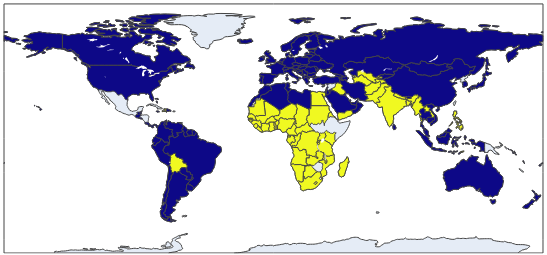
\includegraphics[width=0.8\textwidth]{../images/agglomerative/map-cropped.png}
  \end{figure}
  Cluster 0: Azul; Cluster 1: Amarillo
\end{frame}

% Resultados Gaussian Mixture
\begin{frame}{ResultsGauss}
  \frametitle{Resultados de Gaussian Mixture}
  \begin{figure}
    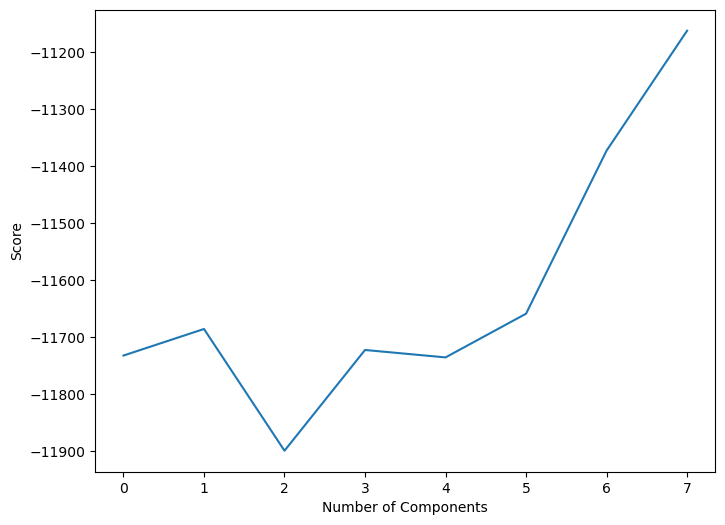
\includegraphics[width=0.8\textwidth]{../images/gaussian/bic.png}
  \end{figure}
\end{frame}

\begin{frame}{ResultsGauss}
  \frametitle{Resultados de Gaussian Mixture}
  \begin{figure}
    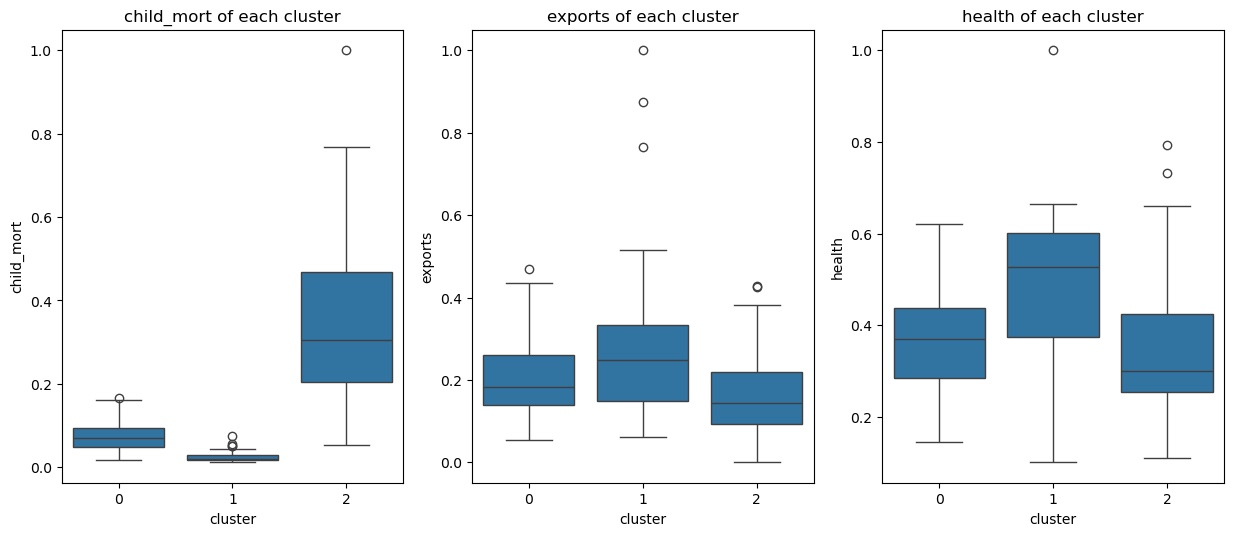
\includegraphics[width=\textwidth]{../images/gaussian/features-dist-1.jpg}
  \end{figure}
\end{frame}

\begin{frame}{ResultsGauss}
  \frametitle{Resultados de Gaussian Mixture}
  \begin{figure}
    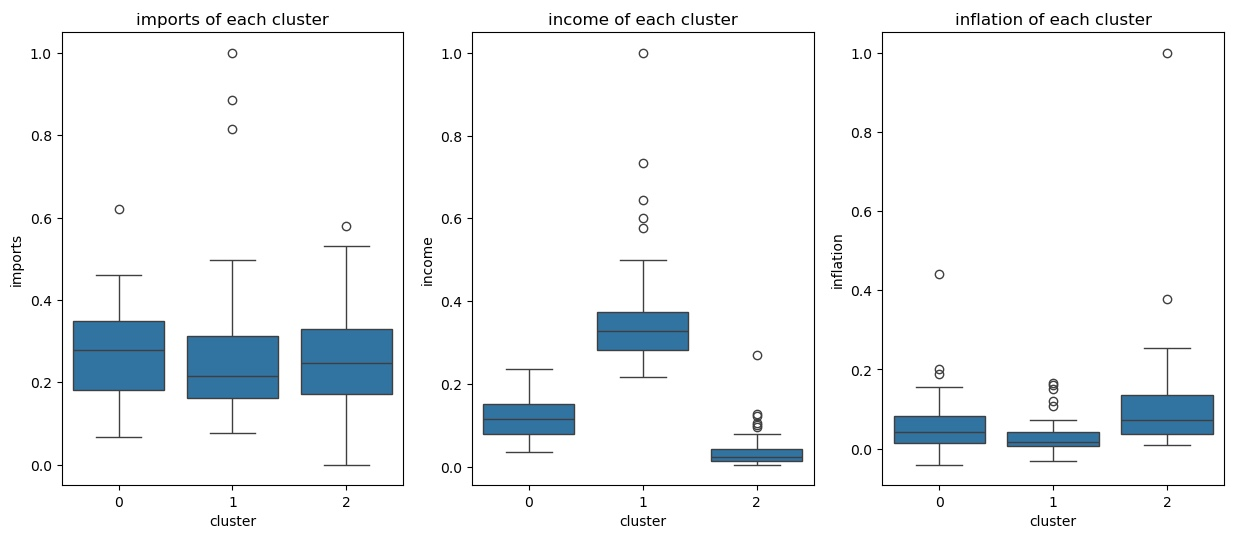
\includegraphics[width=\textwidth]{../images/gaussian/features-dist-2.jpg}
  \end{figure}
\end{frame}

\begin{frame}{ResultsGauss}
  \frametitle{Resultados de Gaussian Mixture}
  \begin{figure}
    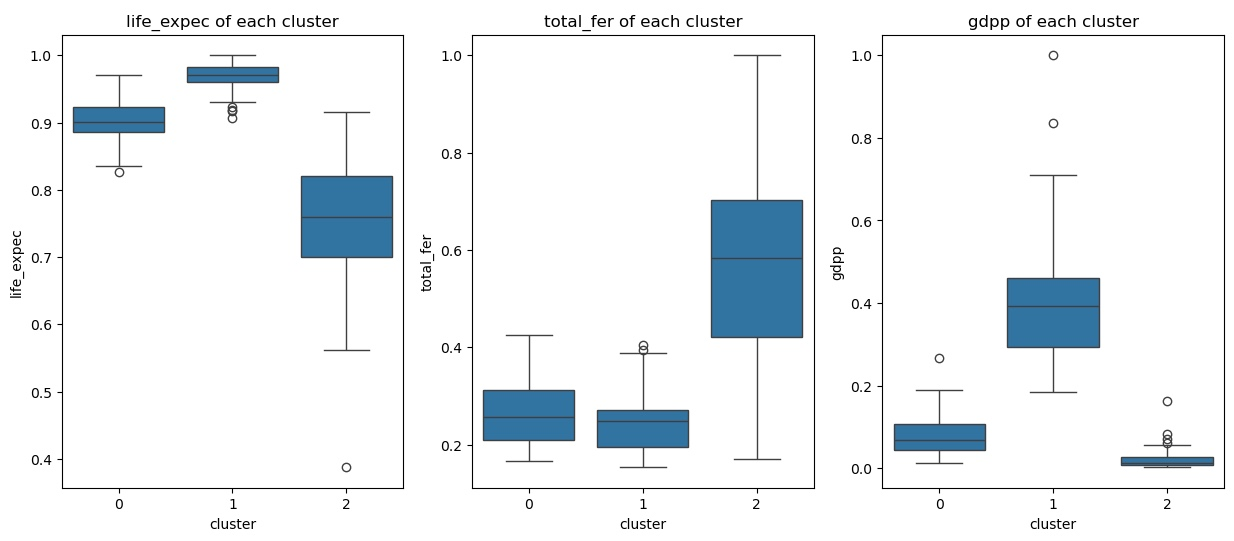
\includegraphics[width=\textwidth]{../images/gaussian/features-dist-3.jpg}
  \end{figure}
\end{frame}

\begin{frame}{ResultsGauss}
  \frametitle{Resultados de Gaussian Mixture}
  \centering
  \begin{figure}
    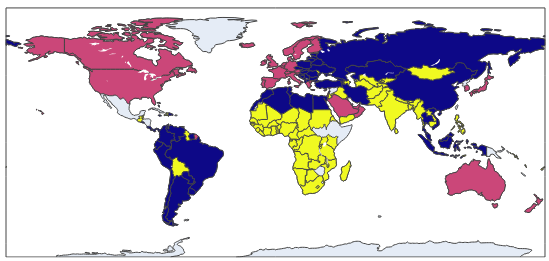
\includegraphics[width=0.8\textwidth]{../images/gaussian/map-cropped.png}
  \end{figure}
  Cluster 0: Azul; Cluster 1: Rosa; Cluster 2: Amarillo
\end{frame}

\begin{frame}{Conclusion}
  \frametitle{Conclusiones}
  \begin{itemize}
    \item \textit{KMeans} y \textit{Agglomerative Clustering} tienen resultados muy similares (distancia euclídea).
    \pause
    \item \textit{KMeans} y \textit{Agglomerative Clustering} incluyen países en vías de desarrollo (Rusia, China...) en el mismo \textit{cluster} que países subdesarrollados (Sudán).
    \pause
    \item \textit{Gaussian Mixture} identifica países desarrollados, en vías de desarrollo y subdesarrollados.
    \pause
    \item Los países en vías de desarrollo se parecen a los desarollados en ámbitos sociales pero a los subdesarrollados en ámbitos económicos.
  \end{itemize}
\end{frame}

\begin{frame}{Conclusion1}
  \frametitle{Conclusiones}
  \centering
  Muchas Gracias!
\end{frame}

\end{document}

